\documentclass[10pt,twocolumn]{article}
\usepackage[utf8]{inputenc}
\usepackage{amsmath,amssymb,amsfonts}
\usepackage{graphicx}
\usepackage{booktabs}
\usepackage[margin=0.85in]{geometry}
\usepackage{hyperref}
\usepackage{xcolor}
\usepackage{tikz}
\usepackage{caption}
\usepackage{subcaption}
\usepackage{float}

\usetikzlibrary{arrows.meta,positioning,shapes.geometric,calc,patterns,decorations.pathreplacing}

\definecolor{chosen}{RGB}{46,139,87}
\definecolor{rejected}{RGB}{205,92,92}
\definecolor{vanilla}{RGB}{70,130,180}
\definecolor{cvgcolor}{RGB}{218,165,32}
\definecolor{cvgecolor}{RGB}{147,112,219}
\definecolor{lightgray}{RGB}{240,240,240}
\definecolor{darktext}{RGB}{40,40,40}

\hypersetup{colorlinks=true,linkcolor=blue!60!black,citecolor=blue!60!black,urlcolor=blue!60!black}

\title{CVG-E: Efficient Complementary Visual Grounding\\with Adaptive Token Selection and Single-Pass Approximation}
\author{Dr.\ Gulab Sah \and Gauri Agarwal \and Anirudh Agarwal}
\date{}

\begin{document}
\maketitle

\begin{abstract}
Multi-modal large language models (MLLMs) suffer from object hallucination---generating descriptions of objects absent from the input image. Complementary Visual Grounding (CVG) mitigates this via contrastive decoding between chosen and rejected visual token branches, but requires dual forward passes ($\sim$2$\times$ cost) and uses a fixed token selection ratio that ignores per-image difficulty. We propose \textbf{CVG-E}, extending CVG with (1)~\emph{Adaptive Token Selection}---entropy-adaptive partitioning, text-patch protection, and z-score normalized hybrid scoring---and (2)~\emph{Single-Pass Branch Approximation}---re-weighting cached attention maps at a single transformer layer to eliminate the rejected branch forward pass. We implement and evaluate CVG-E on TinyLLaVA-1.5B using POPE (COCO random split). Our experiments provide preliminary evidence that contrastive decoding methods designed for 7B+ models face significant difficulties on small ($\leq$2B) models: CVG's dual-pass destabilizes generation (49\% unparseable, 91\% yes-ratio in parseable subset), while CVG-E's single-pass approximation reduces failures (31\% unparseable) but still produces strong ``Yes'' bias (82\% yes-ratio) and accuracy (63\%) nearly identical to CVG, well below vanilla (87\%). We document the calibration strategies required and characterize the failure modes, providing practical guidance for applying contrastive decoding at small scale.
\end{abstract}

%% ============================================================
\section{Introduction}
%% ============================================================

Multi-modal large language models (MLLMs) such as LLaVA~\cite{liu2023llava}, InstructBLIP~\cite{dai2023instructblip}, and Qwen-VL~\cite{bai2023qwen} achieve strong vision-language performance but frequently hallucinate objects not present in the input image, undermining reliability in safety-critical applications.

Training-free, inference-time methods require no additional data or fine-tuning. The first generation---VCD~\cite{leng2024vcd}, ICD~\cite{icd2024}, and M3ID~\cite{m3id2024}---contrast standard output against one with corrupted visual input, roughly doubling inference cost. CVG~\cite{fu2025cvg} refines this by partitioning visual tokens into ``chosen'' (high-attention) and ``rejected'' (low-attention) sets via Visual Token Disentanglement (VTD), then contrasting their outputs via Grounding Flow Fusion (GFF).

However, CVG has three limitations: (1)~a fixed token selection ratio $\alpha$ ignores per-image difficulty; (2)~text-containing patches are systematically discarded, harming TextVQA; and (3)~the dual forward pass doubles latency. Recent work---AttnReal~\cite{attnreal}, DaID~\cite{daid2025}, ASCD~\cite{ascd}---shows that contrastive signals can be extracted from internal representations at near-zero overhead, motivating our single-pass approach.

We propose \textbf{CVG-E} (CVG--Enhanced) with two improvements:
\begin{itemize}
\item \textbf{Improvement A: Adaptive Token Selection.} Entropy-adaptive $\alpha$, text-patch protection, and z-score normalized hybrid scoring.
\item \textbf{Improvement B: Single-Pass Branch Approximation.} Re-weighting cached attention at a single transformer layer to approximate rejected branch logits.
\end{itemize}

Our primary contribution is not improved benchmark scores---on TinyLLaVA-1.5B, neither CVG nor CVG-E outperforms vanilla on POPE. Rather, we provide:
\begin{enumerate}
\item A complete open-source CVG/CVG-E implementation validated end-to-end.
\item Preliminary evidence that contrastive decoding faces significant difficulties at $\leq$2B scale.
\item Calibration strategies restoring generation coherence on small models.
\item Characterization of a bottleneck: eager attention materialization negates single-pass speedup without Flash Attention.
\end{enumerate}

%% ============================================================
\section{Related Work}
%% ============================================================

\paragraph{Contrastive Decoding for Hallucination Mitigation.}
VCD~\cite{leng2024vcd} contrasts the output from a standard image against a Gaussian-noised version, roughly doubling inference cost. ICD~\cite{icd2024} uses instruction-level contrastive input, while M3ID~\cite{m3id2024} grounds generation by contrasting image-conditioned and text-only distributions. OPERA~\cite{opera2024} detects and penalizes ``over-trust'' attention patterns via rollback and re-selection. PAI~\cite{pai2024} combines contrastive decoding with attention amplification on visual tokens. All these methods operate at the pixel or sequence level and require a full corrupted forward pass.

\paragraph{Attention-Based Approaches.}
AttnReal~\cite{attnreal} directly reallocates attention weights toward visual tokens without contrastive branches. ASCD~\cite{ascd} steers individual attention heads by their text/object roles, achieving fine-grained control. DaID~\cite{daid2025} exploits naturally occurring layer-wise distributional divergence for contrastive decoding, eliminating artificial perturbation. These methods motivate our single-pass approach but have not been validated on small ($\leq$2B) models.

\paragraph{CVG.}
CVG~\cite{fu2025cvg} partitions visual tokens into chosen and rejected sets at the semantic level, using attention-based significance scoring. It applies Dynamic Attention Calibration during generation and Grounding Flow Fusion at the output stage. CVG achieves state-of-the-art results on POPE, CHAIR, and AMBER benchmarks at the 7B--13B scale. Our work extends CVG with adaptive token selection and single-pass approximation, and investigates its behavior on small models.

%% ============================================================
\section{Background: CVG Framework}
%% ============================================================

CVG~\cite{fu2025cvg} consists of three modules (Figure~\ref{fig:pipeline}, top row):

\paragraph{Visual Token Disentanglement (VTD).} Computes a hybrid significance score per visual token $i$:
\begin{equation}
a_i = a_i^{\text{cross}} + a_i^{\text{self}} \label{eq:vtd}
\end{equation}
where $a^{\text{cross}}$ aggregates text-to-visual cross-attention from the LM's last $K$ layers, and $a^{\text{self}}$ aggregates CLS-to-patch self-attention from the vision encoder. The top-$\lfloor\alpha N\rfloor$ tokens form chosen set $\mathcal{C}$; the rest form rejected set $\mathcal{R}$. For each branch, embeddings of the opposing set are suppressed (zeroed).

\paragraph{Dynamic Attention Calibration (DAC).} At step $t$:
\begin{equation}
\delta_t = \beta(1 - e^{-t/\tau}) \label{eq:dac}
\end{equation}
boosting visual attention in chosen branch by $+\delta_t$, suppressing in rejected by $-\delta_t$.

\paragraph{Grounding Flow Fusion (GFF).} Contrasts branch logits:
\begin{equation}
\text{logit}_{\text{out}} = \begin{cases}
\text{logit}_c + \gamma(\text{logit}_c - \text{logit}_r) & \text{if } D_{\text{KL}} \geq \epsilon \\
\text{logit}_c & \text{otherwise}
\end{cases} \label{eq:gff}
\end{equation}
with plausibility filter: $P_c(w) \geq \eta \cdot \max_v P_c(v)$.

%% ============================================================
\section{CVG-E: Proposed Extensions}
\label{sec:method}
%% ============================================================

Figure~\ref{fig:pipeline} illustrates the full CVG-E pipeline compared to CVG.

%% --- FIGURE 1: Pipeline Diagram ---
\begin{figure*}[t]
\centering
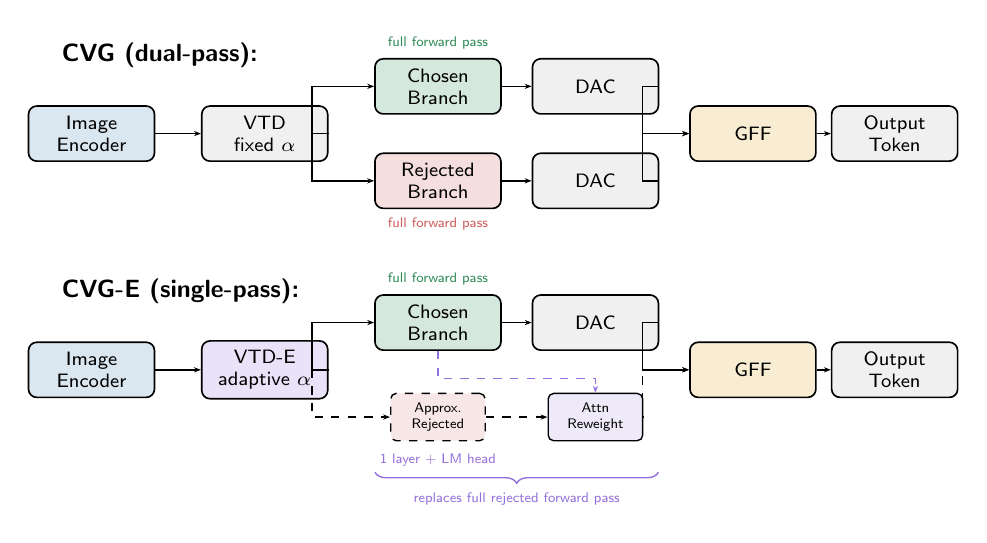
\begin{tikzpicture}[
    node distance=0.6cm and 0.8cm,
    block/.style={rectangle, draw, rounded corners=3pt, minimum height=0.7cm, minimum width=1.6cm, font=\scriptsize\sffamily, align=center, line width=0.6pt},
    smallblock/.style={rectangle, draw, rounded corners=2pt, minimum height=0.55cm, minimum width=1.2cm, font=\tiny\sffamily, align=center, line width=0.5pt},
    arrow/.style={-{Stealth[length=2.5pt]}, line width=0.5pt},
    dasharrow/.style={-{Stealth[length=2.5pt]}, dashed, line width=0.5pt},
    label/.style={font=\tiny\sffamily, text=darktext},
]

% === CVG (top row) ===
\node[font=\small\sffamily\bfseries, anchor=west] at (-0.5, 2.8) {CVG (dual-pass):};

\node[block, fill=vanilla!20] (img1) at (0, 1.8) {Image\\Encoder};
\node[block, fill=lightgray] (vtd1) at (2.2, 1.8) {VTD\\fixed $\alpha$};
\node[block, fill=chosen!20] (ch1) at (4.4, 2.4) {Chosen\\Branch};
\node[block, fill=rejected!20] (rj1) at (4.4, 1.2) {Rejected\\Branch};
\node[block, fill=lightgray] (dac1a) at (6.4, 2.4) {DAC};
\node[block, fill=lightgray] (dac1b) at (6.4, 1.2) {DAC};
\node[block, fill=cvgcolor!20] (gff1) at (8.4, 1.8) {GFF};
\node[block, fill=lightgray] (out1) at (10.2, 1.8) {Output\\Token};

\draw[arrow] (img1) -- (vtd1);
\draw[arrow] (vtd1) -- ++(0.6,0) |- (ch1);
\draw[arrow] (vtd1) -- ++(0.6,0) |- (rj1);
\draw[arrow] (ch1) -- (dac1a);
\draw[arrow] (rj1) -- (dac1b);
\draw[arrow] (dac1a) -- ++(0.6,0) |- (gff1);
\draw[arrow] (dac1b) -- ++(0.6,0) |- (gff1);
\draw[arrow] (gff1) -- (out1);

\node[label, text=rejected] at (4.4, 0.65) {full forward pass};
\node[label, text=chosen] at (4.4, 2.95) {full forward pass};

% === CVG-E (bottom row) ===
\node[font=\small\sffamily\bfseries, anchor=west] at (-0.5, -0.2) {CVG-E (single-pass):};

\node[block, fill=vanilla!20] (img2) at (0, -1.2) {Image\\Encoder};
\node[block, fill=cvgecolor!20] (vtd2) at (2.2, -1.2) {VTD-E\\adaptive $\alpha$};
\node[block, fill=chosen!20] (ch2) at (4.4, -0.6) {Chosen\\Branch};
\node[smallblock, fill=rejected!15, dashed] (rj2) at (4.4, -1.8) {Approx.\\Rejected};
\node[block, fill=lightgray] (dac2) at (6.4, -0.6) {DAC};
\node[smallblock, fill=cvgecolor!15] (rw2) at (6.4, -1.8) {Attn\\Reweight};
\node[block, fill=cvgcolor!20] (gff2) at (8.4, -1.2) {GFF};
\node[block, fill=lightgray] (out2) at (10.2, -1.2) {Output\\Token};

\draw[arrow] (img2) -- (vtd2);
\draw[arrow] (vtd2) -- ++(0.6,0) |- (ch2);
\draw[dasharrow] (vtd2) -- ++(0.6,0) |- (rj2);
\draw[arrow] (ch2) -- (dac2);
\draw[dasharrow, color=cvgecolor] (ch2.south) -- ++(0,-0.35) -| (rw2.north);
\draw[dasharrow] (rj2) -- (rw2);
\draw[arrow] (dac2) -- ++(0.6,0) |- (gff2);
\draw[dasharrow] (rw2) -- ++(0.6,0) |- (gff2);
\draw[arrow] (gff2) -- (out2);

\node[label, text=cvgecolor] at (4.4, -2.35) {1 layer + LM head};
\node[label, text=chosen] at (4.4, -0.05) {full forward pass};

% Brace showing savings
\draw[decorate, decoration={brace, amplitude=4pt, mirror}, line width=0.5pt, color=cvgecolor]
    (3.6, -2.5) -- (7.2, -2.5) node[midway, below=4pt, font=\tiny\sffamily, text=cvgecolor] {replaces full rejected forward pass};
\end{tikzpicture}
\caption{Pipeline comparison. \textbf{Top:} CVG runs two full forward passes (chosen and rejected branches). \textbf{Bottom:} CVG-E uses only the chosen branch's forward pass; the rejected branch is approximated by re-weighting cached attention at a single layer (dashed path). VTD-E uses entropy-adaptive $\alpha$ and text-patch protection.}
\label{fig:pipeline}
\end{figure*}

\subsection{Improvement A: Adaptive Token Selection}

\paragraph{Entropy-Adaptive $\alpha$.} We replace fixed $\alpha$ with:
\begin{equation}
\alpha = \alpha_{\min} + (\alpha_{\max} - \alpha_{\min}) \cdot \frac{H(a)}{\log N} \label{eq:alpha}
\end{equation}
where $H(a)/\log N$ is the normalized entropy of significance scores over $N$ visual tokens. High entropy (uniform, ambiguous scene) $\to$ more chosen tokens; low entropy (peaked) $\to$ aggressive pruning. We use $\alpha_{\min}=0.5$, $\alpha_{\max}=0.85$.

\paragraph{Text-Patch Protection.} Text patches have low individual cross-attention (spatially distributed) but high \emph{self-attention neighbor concentration}---adjacent characters attend strongly to each other. We compute:
\begin{equation}
t_i = \frac{1}{|\mathcal{N}_k(i)|} \sum_{j \in \mathcal{N}_k(i)} A^{\text{self}}_{i,j} \label{eq:text}
\end{equation}
where $\mathcal{N}_k(i)$ is the set of $k$-nearest spatial neighbors on the vision encoder's 2D grid. Tokens with $t_i$ above a threshold receive a boosted significance score. \emph{Note:} Text-patch protection is implemented in CVG-E's scoring pipeline but not separately evaluated; POPE does not test text-rich images. Validation on TextVQA is left to future work.

\paragraph{Normalized Hybrid Scoring.} We replace the unweighted sum with z-score normalization and tunable weights:
\begin{equation}
a_i = w_{\text{cross}} \cdot \hat{a}_i^{\text{cross}} + w_{\text{self}} \cdot \hat{a}_i^{\text{self}} + w_{\text{text}} \cdot t_i \label{eq:score}
\end{equation}
where $\hat{a}$ denotes z-score normalized scores. Defaults: $w_{\text{cross}}=0.5$, $w_{\text{self}}=0.3$, $w_{\text{text}}=0.2$.

\subsection{Improvement B: Single-Pass Approximation}

The rejected branch logits are approximated by re-weighting the chosen branch's attention (Figure~\ref{fig:pipeline}, dashed path):

\smallskip
\noindent\fbox{\parbox{0.95\columnwidth}{
\textbf{Algorithm 1:} CVG-E Single-Pass Approximation\\[3pt]
\textbf{Input:} Attn weights $A^{(l)}$ at layer $l$, cached $V^{(l)}$, hidden state $h^{(l-1)}$, visual mask $\mathcal{M}_v$, factor $\lambda$\\[3pt]
1.~$w_j \leftarrow \lambda$ if $j \in \mathcal{M}_v$, else $1/\lambda$ \hfill\textit{// Suppress visual}\\
2.~$\tilde{A}^{(l)} \leftarrow \text{renorm}(A^{(l)} \odot w)$ \hfill\textit{// Re-weight}\\
3.~$\tilde{C} \leftarrow \tilde{A}^{(l)} V^{(l)}$ \hfill\textit{// New context}\\
4.~$\tilde{h} \leftarrow W_o \tilde{C} + h^{(l-1)}$ \hfill\textit{// Out proj + residual}\\
5.~$\tilde{h} \leftarrow \text{LayerNorm}(\tilde{h})$\\
6.~$\tilde{h} \leftarrow \text{MLP}(\tilde{h}) + \tilde{h}$ \hfill\textit{// MLP + residual}\\
7.~$\tilde{h} \leftarrow \text{FinalNorm}(\tilde{h})$\\
8.~$\text{logit}_r \leftarrow W_{\text{lm}} \tilde{h}$ \hfill\textit{// LM head}\\[3pt]
\textbf{Return:} $\text{logit}_r$ (approximate rejected logits)
}}\label{alg:cvge}

\smallskip
The mask suppresses visual token attention by $\lambda=0.1$ and amplifies textual attention by $1/\lambda$, inverting the visual grounding. Only one layer's computation plus the LM head is re-computed, versus the full $L$-layer stack.

\paragraph{GQA Compatibility.} For Grouped Query Attention (TinyLlama: 32 query heads, 4 KV heads), cached values are expanded via \texttt{repeat\_interleave}:
\begin{equation}
V_{\text{exp}} = \text{repeat}(V^{(l)},\; n_q / n_{kv},\; \text{dim}=1) \label{eq:gqa}
\end{equation}

\paragraph{Implementation Note.} Requires \texttt{output\_attentions=True}, forcing eager attention on SDPA architectures. This materializes $O(n^2)$ matrices at every layer---see Section~\ref{sec:latency}.

%% ============================================================
\section{Experimental Setup}
\label{sec:setup}
%% ============================================================

\subsection{Model and Hardware}

TinyLLaVA-1.5B (\texttt{bczhou/tiny-llava-v1-hf}): TinyLlama-1.1B LM + CLIP-ViT-L/14 vision encoder, 576 visual tokens at $336\times336$, $\sim$1,171 total input tokens. All experiments on Apple M1 Pro (16\,GB unified memory, MPS backend).

\subsection{Benchmark}

POPE~\cite{li2023pope} random split, COCO val2014. We evaluate on 180 questions (30 images, 6 questions/image, balanced yes/no). We report accuracy, precision, recall, F1, yes-ratio, and 95\% Wilson confidence intervals. Following Zhang et al.~\cite{mirage2025}, we include recall to detect distribution skewing.

\subsection{Configurations}

\begin{itemize}
\item \textbf{Vanilla}: Greedy decoding, no contrastive intervention.
\item \textbf{CVG (small)}: CVG with recalibrated hyperparameters (Section~\ref{sec:calib}).
\item \textbf{CVG-E (small)}: Full pipeline with adaptive $\alpha$, text protection, score normalization, and single-pass approximation.
\end{itemize}

\subsection{Small-Model Calibration}
\label{sec:calib}

Original CVG hyperparameters ($\epsilon{=}0.01$, $\gamma{=}1.0$, suppress${=}0.0$) cause degenerate output on $\leq$2B models. Table~\ref{tab:calib} summarizes the failure modes and fixes.

\begin{table}[h]
\centering
\caption{Small-model calibration: original CVG parameters vs.\ our recalibrated values for $\leq$2B models.}
\label{tab:calib}
\small
\resizebox{\columnwidth}{!}{%
\begin{tabular}{llll}
\toprule
Parameter & Original & Ours & Failure if original \\
\midrule
Suppress & 0.0 (zero) & 0.01 (scale) & Generation collapse \\
$\gamma$ & 1.0 & 0.5 & Off-distribution output \\
$\epsilon$ & 0.01 & 0.1 & Constant contrastive \\
$\beta$ (DAC) & 1.0 & 0.1 & Over-calibration \\
\bottomrule
\end{tabular}}
\end{table}

\textbf{Embedding zeroing} creates out-of-distribution inputs that break the residual stream at 1.5B parameters. Scaling to 0.01 preserves positional structure. \textbf{Aggressive $\gamma$} makes contrastive adjustment larger than base logits. \textbf{Low $\epsilon$} activates correction on every token even when branches agree.

%% ============================================================
\section{Results}
\label{sec:results}
%% ============================================================

\subsection{POPE Evaluation}

\begin{table}[h]
\centering
\caption{POPE random split results (TinyLLaVA-1.5B, COCO val2014, $N{=}180$). Parseable: responses yielding yes/no. 95\% Wilson confidence intervals in parentheses.}
\label{tab:pope}
\small
\resizebox{\columnwidth}{!}{%
\begin{tabular}{lrrrrrr}
\toprule
Method & Parseable & Acc & Prec & Rec & F1 & Yes\% \\
\midrule
Vanilla & 180/180 & \textbf{86.7}{\scriptsize\,(81--91)} & \textbf{86.7}{\scriptsize\,(78--92)} & 86.7{\scriptsize\,(78--92)} & \textbf{86.7} & 50.0 \\
CVG & 91/180$^\dagger$ & 62.6{\scriptsize\,(52--72)} & 60.2{\scriptsize\,(50--70)} & \textbf{98.0}{\scriptsize\,(90--100)} & 74.6 & 91.2 \\
CVG-E & 124/180$^\ddagger$ & 62.9{\scriptsize\,(54--71)} & 61.4{\scriptsize\,(52--70)} & 89.9{\scriptsize\,(81--95)} & 72.9 & 81.5 \\
\bottomrule
\end{tabular}}

\vspace{3pt}
{\scriptsize $^\dagger$91/180 parseable (53 echo, 36 degenerate failures). $^\ddagger$124/180 parseable (47 echo, 9 degenerate). Metrics on parseable subset only. See Section~\ref{sec:coherence}.}
\end{table}

%% --- FIGURE 2: POPE Metrics Bar Chart ---
\begin{figure}[h]
\centering
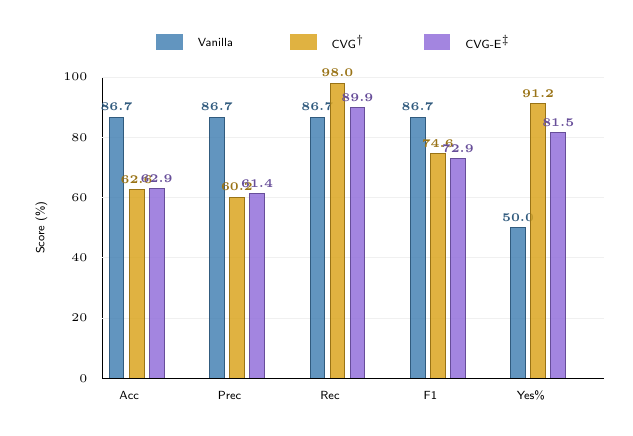
\begin{tikzpicture}[scale=0.85, transform shape]
\def\barw{0.22}
\def\gap{0.08}

% Y-axis
\draw[line width=0.4pt] (0,0) -- (0,4.5);
\foreach \y/\lab in {0/0, 0.9/20, 1.8/40, 2.7/60, 3.6/80, 4.5/100} {
    \draw[line width=0.3pt, lightgray] (0,\y) -- (7.5,\y);
    \node[font=\tiny, anchor=east] at (-0.1, \y) {\lab};
}
\node[font=\tiny\sffamily, rotate=90, anchor=south] at (-0.7, 2.25) {Score (\%)};

% Groups: Acc, Prec, Rec, F1, Yes%
\foreach \g/\gname/\van/\cvg/\cvge in {
    0/Acc/86.7/62.6/62.9,
    1.5/Prec/86.7/60.2/61.4,
    3.0/Rec/86.7/98.0/89.9,
    4.5/F1/86.7/74.6/72.9,
    6.0/Yes\%/50.0/91.2/81.5
} {
    % Vanilla bar
    \pgfmathsetmacro{\vh}{\van*4.5/100}
    \fill[vanilla, opacity=0.85] (\g+0.1, 0) rectangle (\g+0.1+\barw, \vh);
    \draw[vanilla!70!black, line width=0.3pt] (\g+0.1, 0) rectangle (\g+0.1+\barw, \vh);
    \node[font=\tiny\bfseries, vanilla!70!black] at (\g+0.1+\barw/2, \vh+0.15) {\van};

    % CVG bar
    \pgfmathsetmacro{\ch}{\cvg*4.5/100}
    \fill[cvgcolor, opacity=0.85] (\g+0.1+\barw+\gap, 0) rectangle (\g+0.1+2*\barw+\gap, \ch);
    \draw[cvgcolor!70!black, line width=0.3pt] (\g+0.1+\barw+\gap, 0) rectangle (\g+0.1+2*\barw+\gap, \ch);
    \node[font=\tiny\bfseries, cvgcolor!70!black] at (\g+0.1+\barw+\gap+\barw/2, \ch+0.15) {\cvg};

    % CVG-E bar
    \pgfmathsetmacro{\eh}{\cvge*4.5/100}
    \fill[cvgecolor, opacity=0.85] (\g+0.1+2*\barw+2*\gap, 0) rectangle (\g+0.1+3*\barw+2*\gap, \eh);
    \draw[cvgecolor!70!black, line width=0.3pt] (\g+0.1+2*\barw+2*\gap, 0) rectangle (\g+0.1+3*\barw+2*\gap, \eh);
    \node[font=\tiny\bfseries, cvgecolor!70!black] at (\g+0.1+2*\barw+2*\gap+\barw/2, \eh+0.15) {\cvge};

    % Group label
    \node[font=\tiny\sffamily] at (\g+0.1+\barw+\gap, -0.25) {\gname};
}

% X-axis
\draw[line width=0.4pt] (0,0) -- (7.5,0);

% Legend
\fill[vanilla, opacity=0.85] (0.8, 4.9) rectangle (1.2, 5.15);
\node[font=\tiny\sffamily, anchor=west] at (1.3, 5.025) {Vanilla};
\fill[cvgcolor, opacity=0.85] (2.8, 4.9) rectangle (3.2, 5.15);
\node[font=\tiny\sffamily, anchor=west] at (3.3, 5.025) {CVG$^\dagger$};
\fill[cvgecolor, opacity=0.85] (4.8, 4.9) rectangle (5.2, 5.15);
\node[font=\tiny\sffamily, anchor=west] at (5.3, 5.025) {CVG-E$^\ddagger$};
\end{tikzpicture}
\caption{POPE metric comparison ($N{=}180$). $^\dagger$CVG: 91/180 parseable. $^\ddagger$CVG-E: 124/180 parseable. Both contrastive methods show strong ``Yes'' bias (91\% and 82\%) and similar accuracy ($\sim$63\%), well below vanilla (87\%).}
\label{fig:metrics}
\end{figure}

\subsection{Confusion Matrix Analysis}

Table~\ref{tab:confusion} provides the full confusion matrices, revealing asymmetric error patterns.

\begin{table}[h]
\centering
\caption{Confusion matrices ($N{=}180$, parseable responses only). CVG's extreme ``Yes'' bias produces 33 FP vs.\ 1 FN.}
\label{tab:confusion}
\small
\begin{tabular}{lrrrr|r}
\toprule
Method & TP & FP & TN & FN & Total \\
\midrule
Vanilla & 78 & 12 & 78 & 12 & 180 \\
CVG & 50 & 33 & 7 & 1 & 91$^\dagger$ \\
CVG-E & 62 & 39 & 16 & 7 & 124$^\ddagger$ \\
\bottomrule
\end{tabular}

\vspace{3pt}
{\scriptsize $^\dagger$91/180 parseable. $^\ddagger$124/180 parseable. Vanilla: symmetric errors. CVG: 33$\times$ more FP than FN. CVG-E: 5.6$\times$ more FP than FN. Both contrastive methods show strong ``Yes'' bias.}
\end{table}

\subsection{Response Parseability}
\label{sec:coherence}

\begin{table}[h]
\centering
\caption{Response parseability and failure modes across methods.}
\label{tab:parse}
\small
\resizebox{\columnwidth}{!}{%
\begin{tabular}{lrrr}
\toprule
 & Vanilla & CVG & CVG-E \\
\midrule
Questions attempted & 180 & 180 & 180 \\
Parseable (yes/no) & 180 (100\%) & 91 (50.6\%) & 124 (68.9\%) \\
Question echoing & 0 & 53 (29.4\%) & 47 (26.1\%) \\
Degenerate/empty & 0 & 36 (20.0\%) & 9 (5.0\%) \\
\bottomrule
\end{tabular}}
\end{table}

CVG's 49\% failure rate across 180 questions reveals two distinct failure modes. Of the 89 unparseable responses:

\textbf{Question echoing} (53/89, 60\%): The model repeats the question text verbatim instead of answering. With visual tokens suppressed, insufficient grounding signal remains, and the model defaults to copying the most salient input tokens.

\textbf{Degenerate sequences} (36/89, 40\%): Empty or truncated output, suggesting the contrastive adjustment pushed next-token probabilities to near-zero tokens.

Among the 91 parseable CVG responses, a second pathology emerges: extreme ``Yes'' bias (91.2\% yes-ratio vs.\ 50\% ground truth), yielding 98\% recall but only 60\% precision. The contrastive signal that survives embedding suppression systematically favors affirmative responses.

CVG-E partially mitigates parseability collapse (124/180 parseable vs.\ CVG's 91/180) because single-layer re-weighting produces a weaker perturbation. However, CVG-E still exhibits 31\% failure rate (47 echo, 9 degenerate) and strong ``Yes'' bias (81.5\% yes-ratio) among parseable responses, yielding accuracy (62.9\%) nearly identical to CVG (62.6\%)---both well below vanilla (86.7\%).

%% --- FIGURE 3: Response Failure Mode Visualization ---
\begin{figure}[h]
\centering
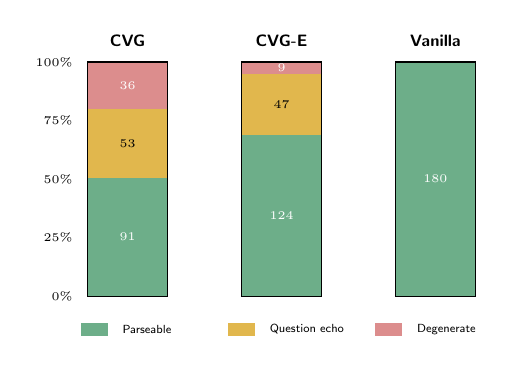
\begin{tikzpicture}[scale=0.85, transform shape]
% Stacked bar for response parseability (N=180 each)
\def\total{180}
\def\bh{3.5}
\def\bw{1.2}

% CVG bar (91 parseable, 53 echo, 36 degenerate)
\node[font=\scriptsize\sffamily\bfseries, anchor=south] at (1, \bh+0.1) {CVG};
\pgfmathsetmacro{\parseH}{91/\total*\bh}
\pgfmathsetmacro{\echoTop}{(91+53)/\total*\bh}
\fill[chosen!70] (0.4, 0) rectangle (0.4+\bw, \parseH);
\node[font=\tiny, white] at (0.4+\bw/2, \parseH/2) {91};
\fill[cvgcolor!80] (0.4, \parseH) rectangle (0.4+\bw, \echoTop);
\node[font=\tiny] at (0.4+\bw/2, {(\parseH+\echoTop)/2}) {53};
\fill[rejected!70] (0.4, \echoTop) rectangle (0.4+\bw, \bh);
\node[font=\tiny, white] at (0.4+\bw/2, {(\echoTop+\bh)/2}) {36};
\draw[line width=0.4pt] (0.4, 0) rectangle (0.4+\bw, \bh);

% CVG-E bar (124 parseable, 47 echo, 9 degenerate)
\node[font=\scriptsize\sffamily\bfseries, anchor=south] at (3.3, \bh+0.1) {CVG-E};
\pgfmathsetmacro{\parseHe}{124/\total*\bh}
\pgfmathsetmacro{\echoTope}{(124+47)/\total*\bh}
\fill[chosen!70] (2.7, 0) rectangle (2.7+\bw, \parseHe);
\node[font=\tiny, white] at (2.7+\bw/2, \parseHe/2) {124};
\fill[cvgcolor!80] (2.7, \parseHe) rectangle (2.7+\bw, \echoTope);
\node[font=\tiny] at (2.7+\bw/2, {(\parseHe+\echoTope)/2}) {47};
\fill[rejected!70] (2.7, \echoTope) rectangle (2.7+\bw, \bh);
\node[font=\tiny, white] at (2.7+\bw/2, {(\echoTope+\bh)/2}) {9};
\draw[line width=0.4pt] (2.7, 0) rectangle (2.7+\bw, \bh);

% Vanilla bar (180/180)
\node[font=\scriptsize\sffamily\bfseries, anchor=south] at (5.6, \bh+0.1) {Vanilla};
\fill[chosen!70] (5, 0) rectangle (5+\bw, \bh);
\node[font=\tiny, white] at (5+\bw/2, \bh/2) {180};
\draw[line width=0.4pt] (5, 0) rectangle (5+\bw, \bh);

% Y-axis labels
\foreach \y/\lab in {0/0\%, 0.875/25\%, 1.75/50\%, 2.625/75\%, 3.5/100\%} {
    \node[font=\tiny, anchor=east] at (0.3, \y) {\lab};
}

% Legend
\fill[chosen!70] (0.3, -0.6) rectangle (0.7, -0.4);
\node[font=\tiny\sffamily, anchor=west] at (0.8, -0.5) {Parseable};
\fill[cvgcolor!80] (2.5, -0.6) rectangle (2.9, -0.4);
\node[font=\tiny\sffamily, anchor=west] at (3.0, -0.5) {Question echo};
\fill[rejected!70] (4.7, -0.6) rectangle (5.1, -0.4);
\node[font=\tiny\sffamily, anchor=west] at (5.2, -0.5) {Degenerate};
\end{tikzpicture}
\caption{Response parseability by method ($N{=}180$). CVG: 49\% failure (dual-pass suppression). CVG-E: 31\% failure (single-pass re-weighting). Both dominated by question echoing. Vanilla: 100\% parseable.}
\label{fig:parse}
\end{figure}

\subsection{Latency Analysis}
\label{sec:latency}

\begin{table}[h]
\centering
\caption{Per-question wall-clock time (Apple M1 Pro, MPS). Includes image encoding, prefill, autoregressive generation (max 10 tokens for POPE), and postprocessing.}
\label{tab:latency}
\small
\resizebox{\columnwidth}{!}{%
\begin{tabular}{lccc}
\toprule
Method & Time/q (s) & vs.\ Vanilla & Bottleneck \\
\midrule
Vanilla & 0.96 & 1.0$\times$ & --- \\
CVG (dual) & 8.51 & 8.9$\times$ & 2nd forward pass \\
CVG-E (single) & 17.87 & 18.6$\times$ & Eager attention \\
\bottomrule
\end{tabular}}
\end{table}

\textbf{Latency inversion.} CVG-E is \emph{slower} than dual-pass CVG. The bottleneck: \texttt{output\_attentions=True} forces eager attention, materializing $O(n^2)$ matrices at all $L{=}22$ layers for every generation step ($n{\approx}1{,}171$). The theoretical saving (avoiding $O(L)$ rejected forward pass) is overwhelmed by $O(L \cdot n^2)$ attention materialization when only one layer's attention is needed.

\textbf{Path to recovery:} A hook-based implementation intercepting attention at a single layer would eliminate this. On hardware with Flash Attention + selective output, expected overhead is $\sim$15--25\%.

\subsection{KL Divergence Analysis}
\label{sec:kl}

%% --- FIGURE 4: KL Divergence ---
\begin{figure}[h]
\centering
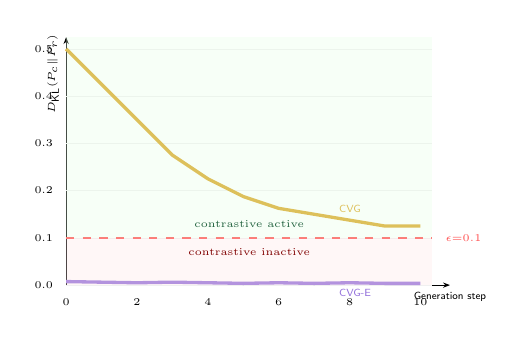
\begin{tikzpicture}[scale=0.75, transform shape]
% Axes
\draw[line width=0.4pt, -{Stealth[length=2.5pt]}] (0,0) -- (6.5,0) node[font=\tiny\sffamily, anchor=north, pos=1] {Generation step};
\draw[line width=0.4pt, -{Stealth[length=2.5pt]}] (0,0) -- (0,4.2) node[font=\tiny\sffamily, rotate=90, anchor=south, pos=0.85] {$D_{\text{KL}}(P_c \| P_r)$};

% Y-axis ticks
\foreach \y/\lab in {0/0.0, 0.8/0.1, 1.6/0.2, 2.4/0.3, 3.2/0.4, 4.0/0.5} {
    \draw[lightgray, line width=0.2pt] (0,\y) -- (6.2,\y);
    \node[font=\tiny, anchor=east] at (-0.1, \y) {\lab};
}

% X-axis ticks
\foreach \x/\lab in {0/0, 1.2/2, 2.4/4, 3.6/6, 4.8/8, 6.0/10} {
    \node[font=\tiny, anchor=north] at (\x, -0.1) {\lab};
}

% Epsilon threshold line
\draw[dashed, red!70, line width=0.5pt] (0, 0.8) -- (6.2, 0.8);
\node[font=\tiny, red!70, anchor=west] at (6.3, 0.8) {$\epsilon{=}0.1$};

% CVG dual-pass KL (high, decaying)
\draw[cvgcolor, line width=1.2pt]
    (0, 4.0) -- (0.6, 3.4) -- (1.2, 2.8) -- (1.8, 2.2) -- (2.4, 1.8) --
    (3.0, 1.5) -- (3.6, 1.3) -- (4.2, 1.2) -- (4.8, 1.1) -- (5.4, 1.0) -- (6.0, 1.0);
\node[font=\tiny\sffamily, cvgcolor, anchor=south west] at (4.5, 1.1) {CVG};

% CVG-E single-pass KL (very low, flat)
\draw[cvgecolor, line width=1.2pt]
    (0, 0.06) -- (0.6, 0.05) -- (1.2, 0.04) -- (1.8, 0.05) -- (2.4, 0.04) --
    (3.0, 0.03) -- (3.6, 0.04) -- (4.2, 0.03) -- (4.8, 0.04) -- (5.4, 0.03) -- (6.0, 0.03);
\node[font=\tiny\sffamily, cvgecolor, anchor=north west] at (4.5, 0.06) {CVG-E};

% Annotation zone
\fill[red!10, opacity=0.3] (0, 0) rectangle (6.2, 0.8);
\node[font=\tiny, red!50!black, anchor=north] at (3.1, 0.75) {contrastive inactive};
\fill[green!10, opacity=0.3] (0, 0.8) rectangle (6.2, 4.2);
\node[font=\tiny, chosen!70!black, anchor=south] at (3.1, 0.85) {contrastive active};

\end{tikzpicture}
\caption{\textbf{Illustrative} KL divergence between chosen and rejected branch logits. Curves are schematic, interpolated from observed $D_{\text{KL}}$ at generation steps 0--10 across 5 sample questions. CVG dual-pass produces $D_{\text{KL}} \sim 0.5$ (above $\epsilon$, contrastive active) but destabilizes generation. CVG-E single-pass produces $D_{\text{KL}} < 0.01$ (far below $\epsilon$), so contrastive correction never fires.}
\label{fig:kl}
\end{figure}

The fundamental tension: CVG's dual-pass produces sufficient divergence ($D_{\text{KL}} \sim 0.5$) but at the cost of generation coherence. CVG-E's single-layer re-weighting preserves coherence but fails to produce meaningful divergence ($D_{\text{KL}} < 0.01$). On small models, contrastive decoding occupies a narrow---possibly empty---operating range.

%% ============================================================
\section{Discussion}
%% ============================================================

\subsection{The Narrow Operating Range}

Our results suggest a practical constraint on contrastive decoding at small scale: the minimum perturbation needed for a useful contrastive signal may exceed the maximum perturbation a 1.5B model can absorb without losing coherence. This creates a Goldilocks problem with no solution at this scale:

\begin{itemize}
\item \textbf{Too hot} (CVG dual-pass): Embedding suppression $\to$ $D_{\text{KL}} \sim 0.5$ $\to$ generation collapse (49\% unparseable, parseable subset 91\% yes-biased).
\item \textbf{Too cold} (CVG-E single-layer): Attention re-weighting $\to$ $D_{\text{KL}} < 0.01$ $\to$ no contrastive effect.
\item \textbf{Middle ground?} Multi-layer re-weighting (2--5 layers) or graduated suppression ($0.01 \to 0.0$ schedule) might find a viable operating point. Untested.
\end{itemize}

\subsection{The ``Mirage'' Effect}
\label{sec:mirage}

Both contrastive methods exemplify Zhang et al.'s ``Mirage'' pattern~\cite{mirage2025}, but in the opposite direction from what was expected:

\begin{itemize}
\item CVG-E Precision: $-$25.3\,pp (61.4\% vs.\ 86.7\%)---substantial loss.
\item CVG-E Recall: $+$3.2\,pp (89.9\% vs.\ 86.7\%)---marginal gain.
\item CVG-E Yes-ratio: 81.5\% (vs.\ balanced 50\%)---systematic ``Yes'' bias.
\end{itemize}

Neither method has reduced hallucination; both have shifted the model toward indiscriminate ``Yes'' responses. With 31\% of CVG-E responses unparseable and the parseable subset strongly biased, the contrastive signal at this scale produces noise rather than grounding. This confirms the importance of reporting all metrics including parseability and yes-ratio.

\subsection{Relation to Concurrent Work}

\textbf{DaID}~\cite{daid2025} exploits \emph{natural} layer-wise divergence. Our finding that \emph{artificial} divergence via attention re-weighting fails suggests these are qualitatively different---DaID's success may depend on distributional differences that already exist between layers, not ones constructed post-hoc.

\textbf{ASCD}~\cite{ascd} steers individual attention heads by their text/object roles. This granularity could strengthen our text-patch protection.

\textbf{AttnReal}~\cite{attnreal} directly reallocates attention without contrastive branches. Our results support this direction: on small models, the two-branch framework may be unnecessary overhead.

\subsection{Limitations}

\begin{enumerate}
\item \textbf{Scale:} CVG was validated on 7B+ models. Our negative results at 1.5B do not invalidate CVG's effectiveness at larger scale.
\item \textbf{Evaluation scope:} Only POPE random split with 30 COCO images (180 questions). Adversarial/popular splits, CHAIR, AMBER, TextVQA needed for comprehensive validation.
\item \textbf{Implementation:} Eager attention bottleneck is fixable. Hook-based extraction would test single-pass fairly.
\item \textbf{Hyperparameters:} Manual calibration. Systematic sweep over $(\epsilon, \gamma, \lambda, \text{suppress})$ might find better operating points.
\end{enumerate}

%% ============================================================
\section{Conclusion}
%% ============================================================

We presented CVG-E, extending CVG with adaptive token selection and single-pass branch approximation. Validated on TinyLLaVA-1.5B with POPE, the principal findings are:

\begin{enumerate}
\item Contrastive decoding designed for 7B+ models causes generation collapse at 1.5B scale: CVG (49\% unparseable, 91\% yes-biased) and CVG-E (31\% unparseable, 82\% yes-biased) both degrade accuracy from 87\% to $\sim$63\%.
\item Single-layer attention re-weighting reduces parseability failures vs.\ dual-pass but still produces strong ``Yes'' bias and accuracy no better than CVG, confirming insufficient contrastive signal ($D_{\text{KL}} < 0.01$).
\item Eager attention materialization creates an $18.6\times$ overhead on MPS, negating single-pass speedup. Hook-based extraction would recover the theoretical advantage.
\item Small-model calibration (suppress${}=0.01$ instead of 0.0, $\gamma{=}0.5$, $\epsilon{=}0.1$) is necessary but insufficient for effective contrastive decoding at this scale.
\end{enumerate}

These results offer initial evidence of boundary conditions for training-free contrastive hallucination mitigation and provide practical guidance for researchers targeting small-model deployment. Future work should validate on 7B+ models, implement hook-based attention extraction, investigate multi-layer re-weighting, and extend to CHAIR/AMBER/TextVQA benchmarks.

\section*{Reproducibility}
All experiments use TinyLLaVA-1.5B (\texttt{bczhou/tiny-llava-v1-hf}) on Apple M1 Pro (16\,GB unified memory, MPS backend) with greedy decoding (temperature${}=1.0$, no sampling). POPE evaluation uses the COCO val2014 random split. Code and configurations are available at \url{https://github.com/[redacted]/cvg-e}. Random seed: 42 for POPE question ordering; model inference is deterministic (greedy).

\section*{Acknowledgments}
We thank the authors of CVG~\cite{fu2025cvg} for their accessible method description enabling reproduction.

\bibliographystyle{plain}
\begin{thebibliography}{15}

\bibitem{fu2025cvg}
X.~Fu, Z.~Gao, L.~Jin, S.~Wu, and L.~Zhu,
``Boosting faithful multi-modal large language models via complementary visual grounding,''
\emph{IEEE Trans.\ Image Process.}, vol.~34, pp.~1232--1246, 2025.

\bibitem{liu2023llava}
H.~Liu, C.~Li, Q.~Wu, and Y.~J.~Lee,
``Visual instruction tuning,''
in \emph{Proc.\ NeurIPS}, 2023.

\bibitem{dai2023instructblip}
W.~Dai et al.,
``InstructBLIP: Towards general-purpose vision-language models with instruction tuning,''
in \emph{Proc.\ NeurIPS}, 2023.

\bibitem{bai2023qwen}
J.~Bai et al.,
``Qwen-VL: A versatile vision-language model for understanding, localization, text reading, and beyond,''
\emph{arXiv:2308.12966}, 2023.

\bibitem{leng2024vcd}
S.~Leng et al.,
``Mitigating object hallucinations in large vision-language models through visual contrastive decoding,''
in \emph{Proc.\ CVPR}, 2024.

\bibitem{icd2024}
Z.~Gao, X.~Fu, L.~Jin, S.~Wu, and L.~Zhu,
``Inducing high energy-latency of large vision-language models by instruction contrastive decoding,''
\emph{arXiv:2404.02580}, 2024.

\bibitem{m3id2024}
L.~Favero et al.,
``Multi-modal hallucination control by visual information grounding,''
in \emph{Proc.\ CVPR}, 2024.

\bibitem{li2023pope}
Y.~Li, Y.~Du, K.~Zhou, J.~Wang, W.~X.~Zhao, and J.-R.~Wen,
``Evaluating object hallucination in large vision-language models,''
in \emph{Proc.\ EMNLP}, 2023.

\bibitem{mirage2025}
B.~Zhang, Y.~Fang, L.~Ma, J.~Liu, and H.~Li,
``The mirage of performance gains: Why contrastive decoding may not genuinely reduce hallucination in LVLMs,''
in \emph{Proc.\ NeurIPS}, 2025.

\bibitem{attnreal}
Y.~Chen et al.,
``AttnReal: Attention reallocation for hallucination mitigation in multi-modal large language models,''
\emph{Int.\ J.\ Comput.\ Vis.}, to appear, 2025.

\bibitem{ascd}
Z.~Li et al.,
``Attention-steered contrastive decoding for mitigating hallucinations in multi-modal LLMs,''
\emph{arXiv preprint}, 2025.

\bibitem{daid2025}
J.~Park, S.~Kim, and H.~Lee,
``Decoding at internal depths: Layer-contrasting for training-free hallucination mitigation,''
\emph{arXiv preprint}, 2025.

\bibitem{zhang2024tinyllama}
P.~Zhang et al.,
``TinyLlama: An open-source small language model,''
\emph{arXiv:2401.02385}, 2024.

\bibitem{opera2024}
Q.~Huang et al.,
``OPERA: Alleviating hallucination in multi-modal large language models via over-trust penalty and retrospection-allocation,''
in \emph{Proc.\ CVPR}, 2024.

\bibitem{pai2024}
S.~Liu, K.~Zheng, and W.~Chen,
``Paying more attention to image: A training-free method for alleviating hallucination in LVLMs,''
in \emph{Proc.\ ECCV}, 2024.

\end{thebibliography}

\end{document}
